\chapter{尿量异常}

健康成人每24小时排尿量在1000~2000ml之间(日尿量与夜尿量之比为2∶1~3∶2),大约相当于每分钟排尿1ml。尿量一般与摄入的水量成正比例。许多情况如饮食、气温、环境、精神紧张、劳动或运动、疼痛等均能影响尿量。如饮大量水、浓茶或咖啡后,尿量增多;高温作业或剧烈运动时,可因大量出汗而使尿量减少。许多病理的情况也能影响尿量,如在糖尿病、尿崩症时,尿量增多;在急性肾炎、急性肾衰竭的早期及少尿期,则尿量减少;当尿路完全梗阻时,则无尿液排出。此等尿量的改变称为尿量异常。

尿量异常可分为少尿或无尿和多尿两种病理情况。

\section{117 少尿或无尿}

24小时内尿量少于400ml或每小时尿量少于17ml者,称为少尿;24小时内尿量少于100ml,或12小时内完全无尿者称为无尿(或尿闭)。

\subsection{(一)少尿或无尿的病因及临床分类}

大致可分为肾前性、肾性及肾后性三大类,其中疾病很多,按表\ref{tab35-1}顺序讨论如下。

\begin{table}[htbp]
\centering
\caption{少尿或无尿疾病的分类}
\label{tab35-1}
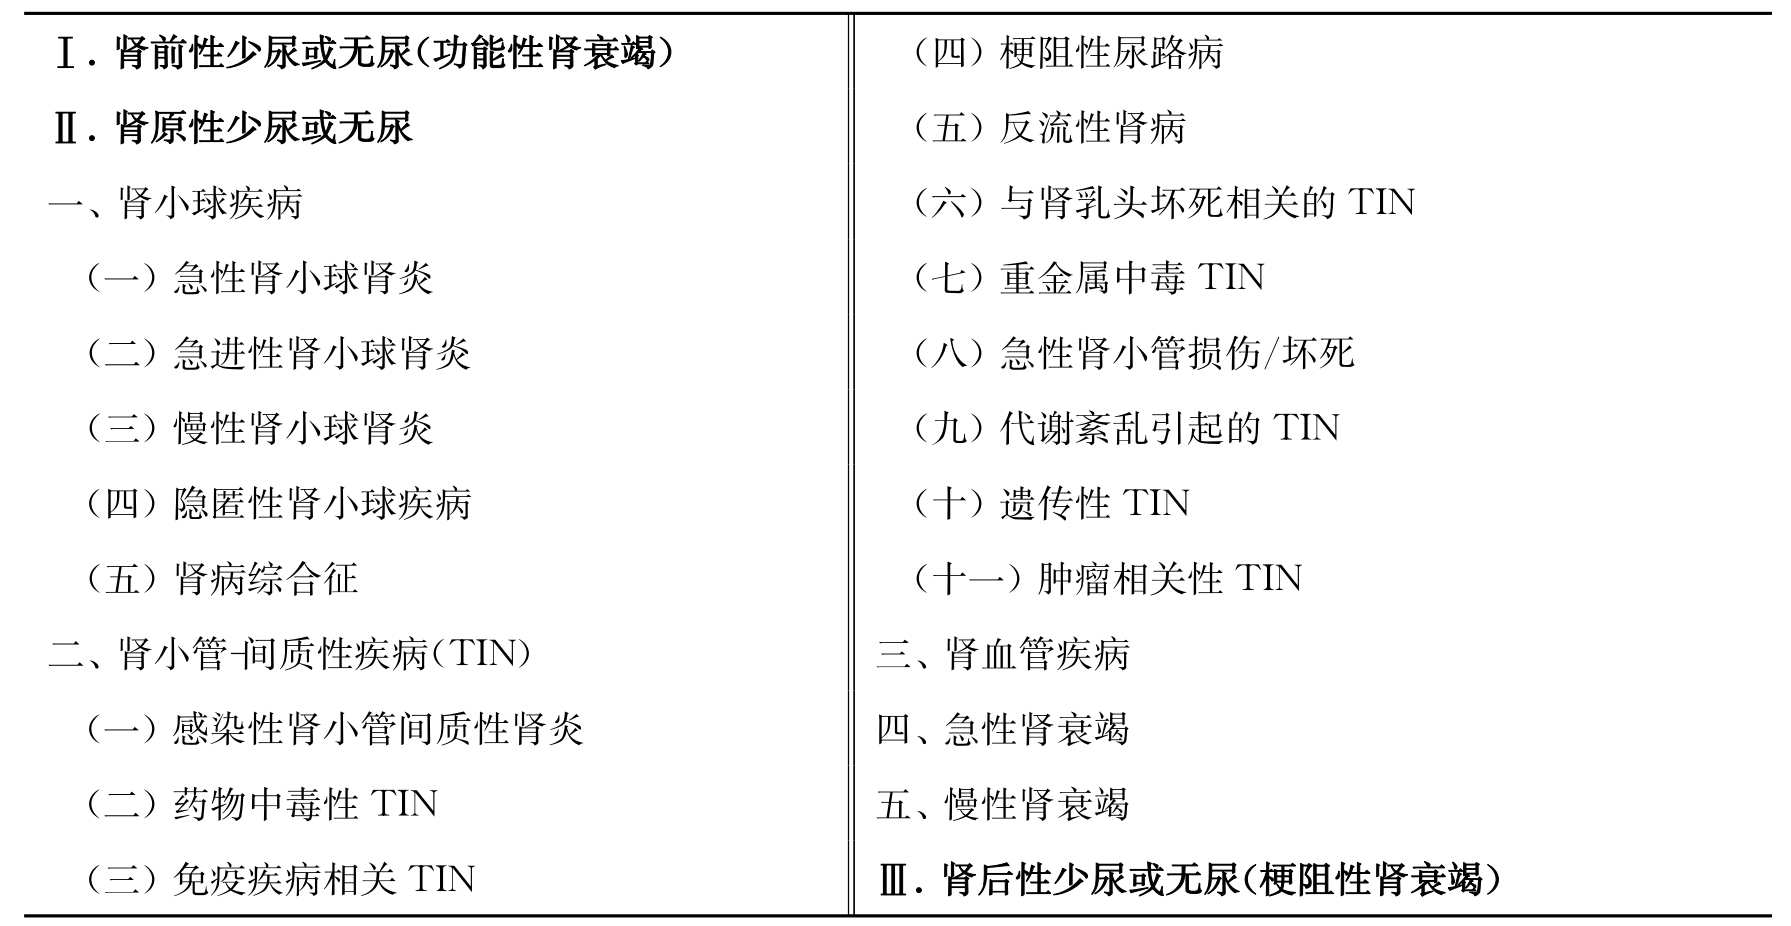
\includegraphics[width=5.95833in,height=3.08333in]{./images/Image00210.jpg}
\end{table}

\subsection{(二)少尿或无尿的诊断和鉴别诊断}

在临床上,当患者12~24小时排尿甚少或无尿排出时,即应考虑少尿或无尿的可能性,但首先应排除机械性下尿路梗阻(如前列腺肥大等)或膀胱功能障碍所致的膀胱尿潴留。当有膀胱尿潴留时,在耻骨上区可见到及摸到膨胀的膀胱,叩诊呈浊音,稍压之,患者有尿意;导尿检查可证实之,且是重要的治疗措施。确定为少(无)尿后,其病因的诊断要根据病史、体征及有关的实验室检查,进行综合性分析、拟诊。

1.肾前性少尿常有引起血容量不足的明确病因(如休克、脱水、心力衰竭等),并有相应的各自特征性的临床表现,尿检查一般较少异常,尿比重>1.020,渗透压>600mOsm/kg。如疾病继续发展可进展为肾性少尿。

2.肾性少尿或无尿导致肾性少尿的病因很多。急性肾小球肾炎与急进性肾小球肾炎起病均较急,均可出现少尿,但急性肾炎的少尿持续时间较短,经1~2周后,尿量会逐渐增多,症状也随之减轻,绝大部分病例可痊愈;而急进性肾炎的少尿持续时间长,病情呈进行性,肾功能急剧恶化,经数周至数月,即进入尿毒症期。慢性肾小球肾炎急性发作所致少尿,可根据患者既往有肾炎病史如水肿、高血压及蛋白尿等,近期内有促发因素存在或肾病本身恶化,一般诊断不难。各种慢性肾脏病所致肾衰竭期的少尿,患者多存在各种肾病的临床特征。但亦有些患者平时无明显肾病表现,在某些应激状态下,可突然发生少(无)尿,类似于急性肾衰竭。这类患者在诊断上应通过详细的询问病史、细致的检查,发现一些慢性肾病的迹象,如水肿、血压高、不可解释的贫血、蛋白尿、血尿、低蛋白血症及长期夜尿增多等,中年以上的患者应注意心、脑、眼底等器官有否动脉硬化表现,同时可选择有关特殊检查以助确诊。双侧肾皮质坏死所致的少(无)尿,因多见于妊娠后期妇女,尤其合并胎盘早期剥离患者,或严重创伤患者,少尿时间长,多出现无尿,肾功能呈进行性急剧恶化,据此可与ATN鉴别。必要时可做肾活检以确诊。重症急性肾盂肾炎、肾乳头坏死的少(无)尿,常伴有高热、明显肾区痛、尿频、尿中白细胞数多,常有白细胞管型,尿细菌检查阳性,肾乳头坏死者可从尿中找到坏死乳头组织块。急性间质性肾炎所致少尿,可根据药物过敏,或感染史。药物过敏引起者可有发热、皮疹、关节痛、血嗜酸性粒细胞增多等,本病与ATN的鉴别诊断较困难,肾活检有助诊断。恶性高血压所致的少(无)尿,多见于患有高血压的中年人,血压明显升高达200/130mmHg以上,常伴有心力衰竭、高血压脑病、视乳头水肿、视网膜出血等全身小动脉受累的表现。至于因系统性红斑狼疮、结节性多动脉炎、其他坏死性血管炎、过敏性紫癜、高尿酸血症、肾动脉血栓形成或栓塞、肾静脉血栓形成、糖尿病、溶血性尿毒症综合征及血栓性血小板减少性紫癜所致的肾损害造成的少(无)尿,可根据原发病的特征性表现进行诊断。

ATN的少(无)尿:患者多有原发病因如休克、中毒、严重感染、外伤或血管内溶血等,一般诊断不难。但常需与肾前性(功能性)少尿相鉴别,因两者的治疗和预后完全不同,及时诊断十分重要。这时可根据患者的血生化和尿改变鉴别(表\ref{tab35-2})。

3.肾后性少尿或无尿在临床上,如患者原来尿量正常而突然出现完全无尿,或少(无)尿与多尿交替出现,则应考虑肾后梗阻性少(无)尿。如伴有肾绞痛、血尿或肾盂积液,或触到肿大的肾脏,一般诊断容易确立。对诊断困难的病例或需要明确梗阻的部位,可作腹部平片、静脉肾盂造影、逆行肾盂造影、放射性核素肾图、B超或CT等以助诊断。

现就主要的疾病讨论如下:

\protect\hypertarget{text00270.html}{}{}

\subsection{一、肾前性少尿或无尿}

肾前性少尿或无尿的常见病因有:休克、低血压、心功能不全、脱水与电解质紊乱、重症肝病(如黄色肝萎缩、肝衰竭、肝肾综合征等)、重症低蛋白血症等,偶也可见于双侧肾动脉血栓形成、栓塞或严重狭窄等。这些病因可引起全身有效血容量减少,及(或)肾血液灌流量不足;肾小球有效滤过压降低,肾小球滤过率减少,导致尿量减少,甚至无尿。同时,可伴有继发性醛固酮增多,血管升压素分泌增加及交感神经兴奋等因素参与,使尿量更加减少。若这些因素能及时得以纠正,血容量或肾血液灌流量恢复正常后,尿量可迅速复原,否则可进一步发展为肾性少尿。

肾前性少尿或无尿的临床特点是:尿量仅为轻度或中度减少,一般不会出现无尿,尿比重增高(在1.020以上),渗透压升高;此时不存在肾实质损伤,当病因已矫治,血压或血容量恢复正常后尿量可迅速增多。在临床上患者有上述病史存在,而出现尿少时,即应考虑肾前性少尿的可能。对于休克或严重脱水所致少尿,应注意与急性肾衰竭相区别。因前者常是急性肾衰竭的早期表现,如病情严重,治疗不及时或不恰当,可使病势进展而成为急性肾衰竭(ARF)。表\ref{tab35-2}可供参考。

\begin{table}[htbp]
\centering
\caption{急性肾衰竭与肾前性少尿或无尿的鉴别}
\label{tab35-2}
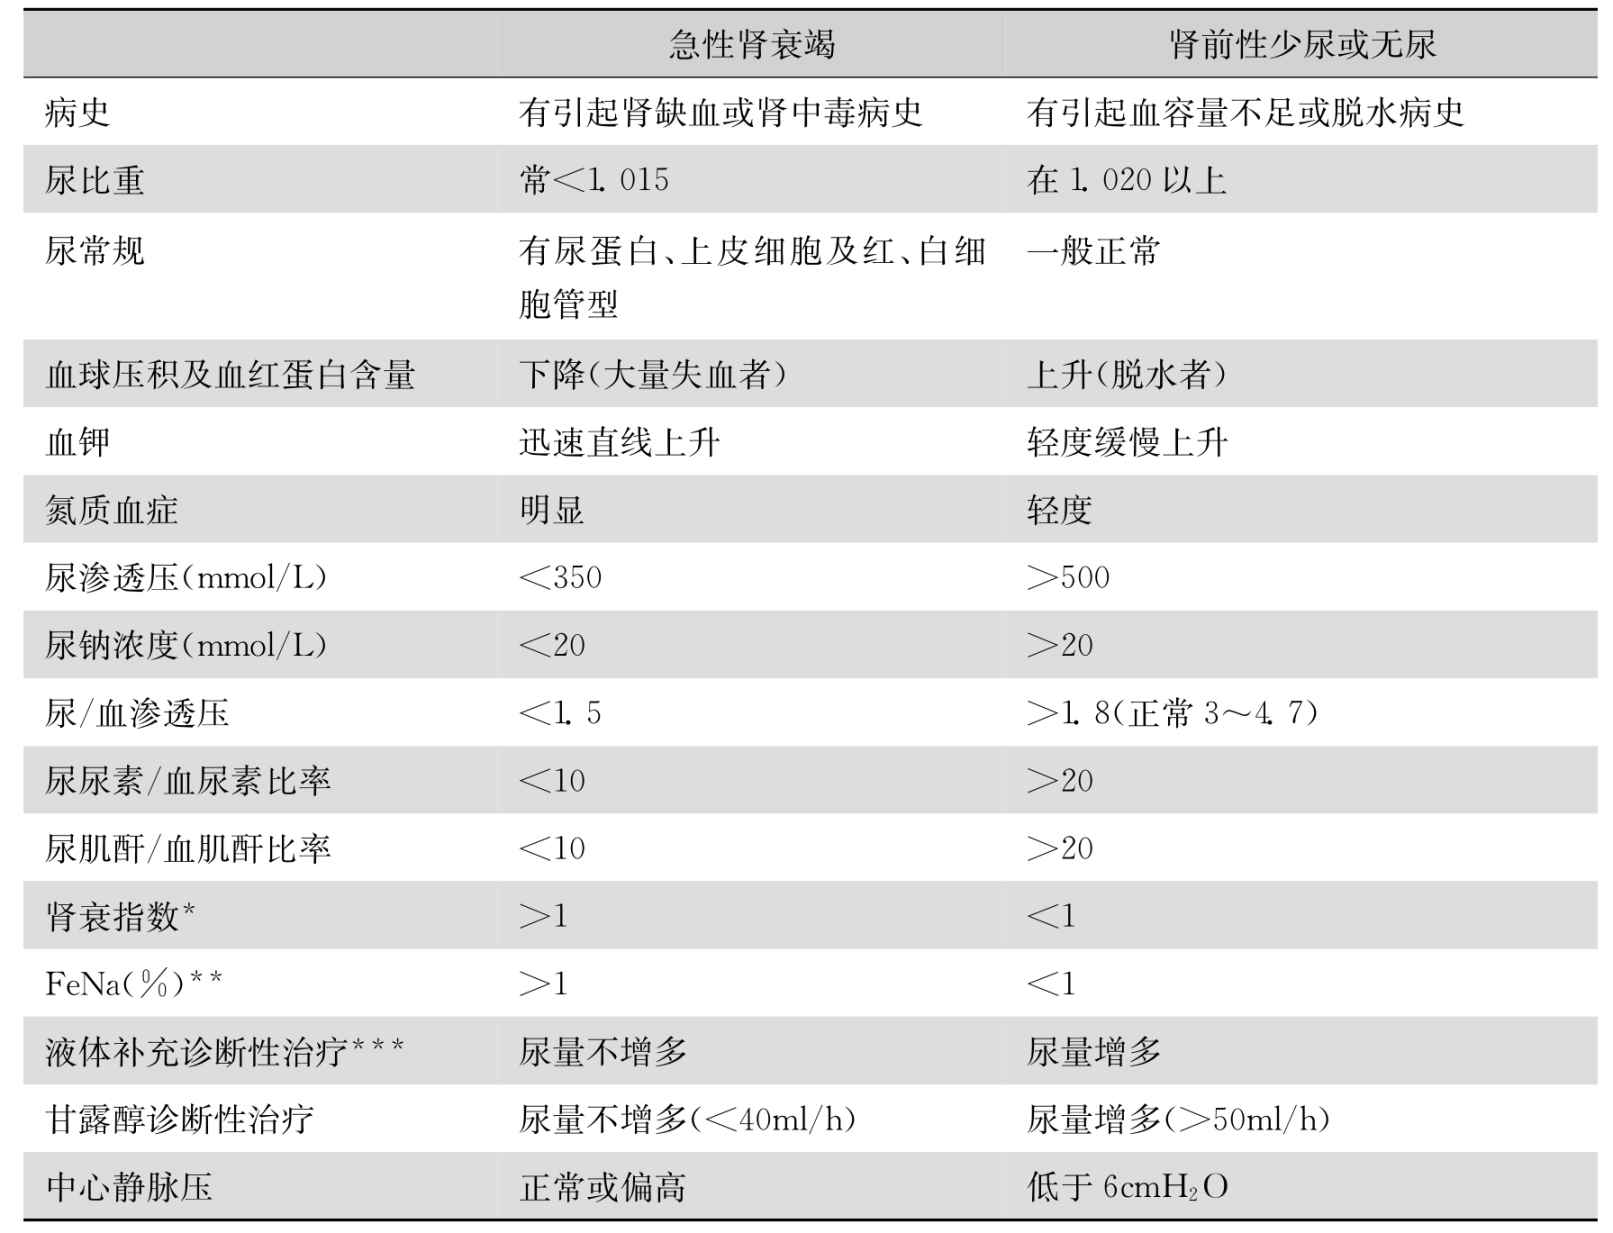
\includegraphics[width=5.95833in,height=4.55208in]{./images/Image00211.jpg}
\end{table}

*肾衰指数:尿钠(mmol/L)/尿肌酐和血肌酐的比数

**FeNa(\%)=$\frac{\text{尿}\ce{Na+}/\text{血}\ce{Na+}}{尿肌酐/血肌酐}$

***液体补充诊断性治疗
用500ml液体于30~40分钟静脉滴完。选择液体因病而异,失血者用全血,烧伤者用血浆或右旋糖酐,失水失盐者用生理盐水,单纯失水者用5\%葡萄糖液。此法易导致心肺功能不全,故应严格掌握适应证,主要适用于临床上认为有血容量不足者,在高度怀疑急性肾衰竭者,一般不宜采用

\protect\hypertarget{text00271.html}{}{}

\subsection{二、肾性少尿或无尿}

\subsubsection{(一)肾小球疾病}

可分为原发性、继发性和遗传性。原发性肾小球疾病的病因未明,继发性肾小球疾病系指全身性疾病(如系统性红斑狼疮、糖尿病、过敏性紫癜等)所致的肾小球损害,遗传性肾小球病为遗传变异基因所致的肾小球疾病(如Alport综合征等)。尽管病因不同,但它们可有相似的临床表现,下文着重介绍原发性肾小球疾病。

\paragraph{1.急性肾小球肾炎}

急性肾小球肾炎(简称急性肾炎)由于肾小球急性炎症,滤过膜被损害,肾内小动脉发生收缩,毛细血管腔变窄、阻塞,导致GFR下降,而肾小管病变较轻,重吸收功能相对尚好;造成所谓球-管失衡,以致少尿。这种少尿的特点是高渗性少尿(比重>1.018,渗透压>600mOsm/kg)。

本病诊断依据为:

(1)部分病例有急性链球菌感染或其他病原微生物感染史,多在感染后1~3周发病。

(2)尿改变有血尿、蛋白尿、管型尿(如红细胞管型、颗粒管型等)。

(3)临床表现常有高血压及水钠潴留现象(如水肿等)。可有短暂的氮质血症。

(4)B超示双肾无缩小。

\paragraph{2.急进性肾小球肾炎}

急进性肾小球肾炎(简称急进性肾炎)引起少尿的原因主要是由于广泛的肾小球(>50\%)的球囊腔内大新月体形成,GFR进行性降低所致。其少尿的特点与急性肾炎综合征相似,但呈进行性少(无)尿。

本病诊断依据为:

(1)起病急、病情重、进展迅速,多在发病数周或数月之内出现较重的肾功能损害。

(2)临床表现一般有明显的水肿、蛋白尿、血尿、管型尿等。也常有高血压、低蛋白血症及迅速发展的贫血。

(3)肾损害常呈进行性加重,多早期出现少尿或无尿。

(4)病理为新月体肾小球肾炎。

\paragraph{3.慢性肾小球肾炎}

慢性肾小球肾炎(简称慢性肾炎)的诊断依据为:

(1)起病缓慢,病情迁延,病情进展可出现肾功能减退、贫血、电解质紊乱等情况。

(2)可有不同程度的水肿、高血压、蛋白尿、血尿、管型尿,部分或全部出现。

(3)病程中可有肾炎急性加重,可能由于某种应激因素(如严重感染、休克,失血或脱水与电解质紊乱、手术、外伤、各种过敏与中毒等)加重肾负担所致;也可能是原来肾小球病变加重或广泛新月体形成,使原来代偿的肾功能呈急剧恶化,导致GFR明显降低,而发生少尿或无尿。

\paragraph{4.隐匿性肾小球疾病}

隐匿性肾小球疾病(无症状血尿或蛋白尿)的诊断依据为:

(1)患者无急、慢性肾炎及其他肾脏病病史,肾功能基本正常。

(2)患者无明显临床症状与体征,临床表现为单纯性蛋白尿或(及)肾小球性血尿。

(3)除外非肾小球性血尿与功能性血尿。

此型肾炎一般不出现尿量减少。

\paragraph{5.肾病综合征}

肾病综合征的诊断依据为:

(1)大量蛋白尿。24小时尿蛋白定量>3.5g。

(2)低蛋白血症。血浆白蛋白浓度<30g/L。

(3)水肿。

(4)高脂血症。

其中第(1)、(2)项为必需。重症肾病综合征的患者可出现尿量减少。

\subsubsection{(二)肾小管间质性肾炎(TIN)}

可分为急性小管间质性肾炎(AIN)和慢性小管间质性肾炎(CIN),AIN常出现少尿或非少尿性急性肾衰竭,而CIN则多表现为夜尿多,低比重和低渗透压尿。急性小管间质性肾炎出现尿少的原因主要是由于肾间质炎症、水肿、出血等使肾小球囊内压升高,致GFR减低;同时,肾小管上皮细胞坏死,引起原尿回漏、管腔阻塞,妨碍原尿排出,引起少尿。

肾小管间质性疾病(TIN)于1985年WHO曾制定新的分类方法,值得参考,简介如下:

\paragraph{1.感染性肾小管间质性肾炎}

感染性肾小管间质性肾炎病原为急性细菌性肾盂肾炎、全身性感染的直接蔓延、特异性感染(如结核、麻风、梅毒)等。

\paragraph{2.药物介导性TIN}

药物介导性TIN可为急性或慢性。急性病例通常是由于药物直接对肾小管的毒性损害或过敏反应所致。前者主要表现为急性肾小管损伤或坏死,而药物过敏性TIN临床上可表现为发热、恶心呕吐、急性肾功能不全、镜下或肉眼血尿、血沉加快、皮疹及血象嗜酸性粒细胞增多等。

药物介导性TIN较轻者引起急性肾小管损伤(ATD),表现为肾小管功能障碍引起的电解质紊乱(低钾血症、高钾血症、低钠血症)以及肾小管酸中毒等。而损害严重时则可引起急性肾小管坏死(ATN),导致少尿、无尿的严重情况。肾毒性药物主要有氨基糖苷类、万古霉素、头孢菌素类、两性霉素B、环孢素类、转换酶抑制剂、利尿剂(氨苯蝶啶、呋塞米等)、非甾体消炎药物(吲哚美辛、保泰松、布洛芬等)、抗肿瘤药物(如顺铂、卡莫司汀、丝裂霉素等)、重金属等。此外,碘造影剂也可以引起肾小管间质损害。

\paragraph{3.免疫疾病相关性TIN}

免疫疾病相关性TIN由于不同的免疫学机制可通过相同的介质导致组织损伤,因而相关致病因子的识别是免疫疾病相关性TIN正确分类的最可靠依据。

\paragraph{4.梗阻性尿路病}

梗阻性尿路病是尿路梗阻引起的结构改变,其症状与体征取决于梗阻发生的原因、部位、持续时间、严重程度以及是否合并尿路感染及肾脏损害等。其病理改变为肾盂积水、肾盏扩张、肾皮质萎缩及肾间质纤维化。如并发感染,则出现急、慢性肾盂肾炎的病象。B超、X线等影像学检查有助于诊断。

\paragraph{5.反流性肾病}

反流性肾病指膀胱输尿管尿液反流引起的肾皮髓质瘢痕化。诊断通常是依据膀胱镜及影像学检查而确定。根据排尿性膀胱尿路造影本病可分为五级:Ⅰ级:造影剂反流只达到输尿管;Ⅱ级:造影剂反流到输尿管、肾盂及肾盏,但肾盏或输尿管无扩张;Ⅲ级:输尿管轻度或中度扩张及(或)扭曲,肾盂轻度或中度扩张,但无或仅有轻度肾盏变钝;Ⅳ级:输尿管中度扩张及(或)扭曲,肾盂中度扩张,肾盏锐角完全消失,但大部分肾盏保持乳头压痕;Ⅴ级:输尿管严重扩张和扭曲,肾盂肾盏严重扩张,大部分肾盏不能见到乳头压痕。

\paragraph{6.与肾乳头坏死相关的TIN}

在本组病例中,糖尿病肾病与止痛剂肾病的肾乳头坏死的鉴别较为重要。前者通常呈急性,病情重,预后差,肾盂造影显示单侧或双侧多个肾乳头处于同一坏死阶段。组织学上肾乳头坏死的周边有中性粒细胞浸润带,但无囊性变,钙化罕见,并可见到糖尿病肾病肾小球损伤的改变。而止痛剂肾病经过慢性,常反复发作,预后较好;肾盂造影几乎两侧所有肾乳头均受累,且处于不同坏死阶段。组织学上肾乳头坏死的周边无中性粒细胞浸润带,坏死区由肾乳头末端向髓质延伸,常见钙化。坏死肾乳头覆盖的皮质区呈慢性TIN改变。

\paragraph{7.重金属中毒TIN}

此组患者常有重金属接触史。一次大剂量接触可导致急性肾衰竭,长期接触可引起慢性小管间质性肾炎。组织学上比较具有特征的重金属中毒性TIN,是急性或亚急性铅中毒,肾小管细胞核内出现圆形嗜伊红性包涵体。急性汞中毒则表现为典型的急性肾小管坏死,以近端小管病变最为明显。此外,镉、金、锂、砷、铜、铂等重金属也可引起中毒性TIN。需要指出的是,顺铂作为一种有效的抗癌药物,亦可引起类似其他重金属的肾脏损害。顺铂用量过大时可引起肾小管变性坏死而导致急性肾衰竭。慢性顺铂中毒晚期可出现钙化管型及间质炎性纤维化。

\paragraph{8.急性肾小管损伤/坏死}

本组TIN主要是指中毒、肾缺血、异型输血后溶血及严重肌肉损伤释出肌红蛋白等所致的急性肾小管坏死。详见本章急性肾衰竭。

\paragraph{9.代谢紊乱引起的TIN}

当血钙>2.75mmol/L时可引起高钙血症性肾病,常见钙管型,肾小管基膜及肾间质内钙沉积。尿酸盐肾病或草酸盐肾病在集合管内可见到尿酸盐或草酸盐结晶沉积。其他代谢性肾病通过肾活检组织学检查亦多能确定诊断。必须指出,代谢紊乱引起的TIN多为慢性,临床上多表现为夜尿多,低比重和低渗透压尿。

\hypertarget{text00271.htmlux5cux23CHP35-1-4-2-10}{}
10.遗传性TIN

此组疾病包括髓质囊性病,病因不明的家族性间质性肾炎及Alport综合征。患者家族史、家系调查及基因诊断,有助于确定。

\hypertarget{text00271.htmlux5cux23CHP35-1-4-2-11}{}
11.肿瘤相关性TIN

此类患者具有恶性肿瘤的临床表现、实验室检查及影像学检查特点。组织学检查对建立诊断甚有帮助。骨髓瘤肾病的病理改变是在远端小管和集合管出现大量的层状透明管型,周围常有上皮或多核巨细胞包绕,近端小管内可见大量透明小滴。轻链肾病则表现为近端小管细胞内包涵体及肾小管与肾小球基膜上线性沉积物,免疫荧光显示沉积物主要由κ或λ链组成。

\subsubsection{(三)肾血管疾病}

包括肾脏的大血管疾患及原发性和继发性肾小血管炎肾损害。前者见于一侧或两侧肾动脉栓塞或肾静脉血栓形成;后者见于各种原发性或继发性肾小血管的坏死性、过敏性血管炎以及恶性高血压所致的小血管炎。此外,妊娠子痫、胎盘早剥、溶血性尿毒症综合征、DIC等也可由于血栓性微血管病导致肾损害。上述原因的肾血管疾患均可引起肾小球滤过率急剧下降而出现少尿或无尿。

\subsubsection{(四)急性肾衰竭(ARF)}

急性肾衰竭是由各种原因引起的肾功能在短时间(几小时至几天)内突然下降而出现的临床综合征。主要表现为血肌酐和尿素氮进行性上升,水电解质和酸碱平衡紊乱,常伴有少尿或无尿,但也可以无少尿表现。急性肾衰竭患者血肌酐平均每日增加≥44.2mmol/L。

急性肾衰竭有广义和狭义之分,广义的急性肾衰竭可分为肾前性、肾性和肾后性。狭义的急性肾衰竭是指急性肾小管坏死(ATN),是肾性急性肾衰竭最常见的类型。

引起ATN的原因很多,文献报道达100余种,主要为:

\paragraph{1.严重肾缺血、缺氧}

主要由于急性循环衰竭,如各种原因的休克、严重的创伤、大面积烧伤、严重的水电解质紊乱(如重度脱水)以及严重急性感染等。

\paragraph{2.急性血管内溶血}

如血型不相合的输血、黑尿热、蚕豆病等。

\paragraph{3.肾中毒}

特别是肾毒性药物如氨基糖苷类抗生素、头孢菌素类抗生素、万古霉素等,或药物过敏反应,均可引起急性肾衰竭。

其他如重金属、生物毒素(蛇毒、蕈毒、棉酚、蜂毒、鱼胆汁)导致急性肾衰竭者也有报道。

急性肾衰竭出现少尿的机制是由于肾缺血(尤其肾皮质),入球小动脉痉挛,肾小球毛细血管内皮肿胀,肾间质水肿,肾小球囊内压升高,导致GFR极度下降(常<5ml/min)。此外,肾小管上皮细胞因缺血或毒素作用而坏死,管壁溃破,致原尿外溢,渗向肾间质;脱落的上皮细胞聚结或因色素管型(如血红蛋白、肌红蛋白)等阻塞管腔,使原尿不能排出。这些因素的共同作用,乃引起少(无)尿。这种少尿的特点是低渗性少尿(尿比重<1.015,渗透压300~400mOsm/kg)。

急性肾衰竭诊断依据:

1.既往无肾病史,发病前有明确病因(如肾缺血或肾中毒)。

2.短时间内肾小球滤过率进行性下降,血清肌酐和尿素氮迅速明显上升,平均每日增加44.2~88.4mmol/L和3.6~7.1mmol/L。高分解代谢者,血肌酐和尿素氮升幅更高。

3.补液扩容,纠正心衰后,尿量仍不增加。

4.尿比重低而固定,等渗尿,尿钠>20mmol/L,FeNa>1\%,肾衰指数>1。

5.排除肾前性、肾后性因素。

必须注意,排除了肾前性和肾后性因素后,对原因不明的急性肾衰竭患者,肾活检病理检查对诊断和治疗均有很大价值。

此时应每日(甚至每小时)检测尿量,并作准确的尿比重测量。如患者原先并无心、肾疾病,而血容量估计已经补足,但患者仍尿量少(<40ml/h),且尿比重低于1.018时,应高度警惕ARF。如尿比重低于1.015更有诊断价值。患者尿有蛋白,尿沉渣镜检可见红细胞、白细胞、肾上皮细胞管型及/或肾衰竭管型等。

\subsubsection{(五)慢性肾衰竭}

慢性肾衰竭是慢性肾脏疾病或累及肾脏的系统性疾病所致的慢性肾功能减退,以及由此产生的各种临床症状与代谢紊乱所组成的综合征。慢性肾衰竭进展至肾衰竭期和尿毒症期,由于GFR极度降低,可出现少尿或无尿。其少尿的特征为低渗性少尿,尿比重低而固定(在1.010左右)。如患者既往有长期慢性肾病史,有慢性肾衰竭各系统表现者,诊断不难。对过去病史不明者,有时需与急性肾衰竭鉴别,尿毒症面容,贫血、高磷血症、低钙血症、血PTH水平升高、影像学检查提示双肾缩小,均支持慢性肾衰竭的诊断。

慢性肾衰竭一般可区分为四期:

1.肾功能不全代偿期肾小球滤过率(GFR)50~80ml/min(临床常用肌酐消除率代表GFR)。血清肌酐(Scr)133~177μmol/L。临床无症状。

2.肾功能不全失代偿期(氮质血症期)GFR 50~20ml/min,Scr
186~442μmol/L。临床出现乏力、轻度贫血、食欲减退等症状。

3.肾衰竭期GFR 20~10ml/min,Scr
451~707μmol/L。临床上出现贫血,钙磷代谢紊乱、水电解质紊乱、酸中毒等。

4.尿毒症期或肾衰竭终末期GFR<10ml/min,Scr>707μmol/L。全身各系统症状明显。

\subsubsection{(六)肾移植后急性排异反应}

主要是由于免疫反应,致GFR下降而产生少尿。

\protect\hypertarget{text00272.html}{}{}

\subsection{三、肾后性少尿或无尿(梗阻性肾衰竭)}

肾后性少尿或无尿,基本上属外科范畴。一切导致尿路梗阻的原因均可能发生肾后性少尿或无尿。

诊断主要依据:

1.有导致尿路梗阻的原发病如结石、肿瘤、前列腺肥大,输尿管瘢痕性狭窄等病史。

2.少尿或无尿常突然发生。

3.可有肾绞痛,胁腹或下腹部疼痛,肾区叩痛。

4.B超、CT、MRI等影像学检查可帮助确诊,常显示肾脏体积增大,肾盂、肾盏、输尿管扩张、积液。并可显示盆腔及腹后壁肿块、输尿管结石等病变。

5.逆行输尿管造影对诊断也有帮助,输尿管肾盂镜对诊断与治疗上尿路梗阻性疾病效果满意。

\protect\hypertarget{text00273.html}{}{}

\section{118 多尿}

24小时尿量经常超过2500ml以上者,为多尿。健康人当饮水过多或食用含水分较多的食物时,可出现暂时性生理性多尿现象。此外,黏液性水肿患者应用甲状腺素治疗时、水肿患者应用利尿剂时、充血性心力衰竭患者在使用洋地黄类或利尿药物治疗时、巨大肾盂积水突然通畅时,也能出现暂时多尿现象。

\subsection{【多尿的病因和临床分类】}

能引起多尿的疾病很多(表\ref{tab35-3})。

多尿的产生一般认为与下列因素有关:

\subsubsection{(一)内分泌代谢功能障碍}

①尿崩症:是由于原发性或继发性下丘脑-神经垂体损害,血管升压素(ADH)分泌减少或缺如,影响远端肾小管及集合管对水分重吸收而致多尿;②糖尿病:是由于血糖过高,肾小球滤过的糖增多,尿中含糖高,肾小管腔内渗透浓度增高,限制了水分的重吸收,因而出现多尿,多饮也是其重要原因之一;③原发性甲状旁腺功能亢进:是由于甲状旁腺激素分泌增多,引起持续性高钙血症,引起烦渴、多饮,同时可损害肾小管的浓缩功能,加之近端肾小管重吸收磷酸根也受抑制,大量磷酸根从尿中排出而引起多尿;④原发性醛固酮增多症:是由于肾上腺皮质分泌醛固酮增多,作用于远端小管,而起潴钠排钾作用,血钠增高刺激下视丘口渴中枢而致烦渴、多饮引起多尿;另一方面也可因从尿中大量失钾,引起严重低钾血症,以致失钾性肾炎,影响小管-间质的浓缩尿液的功能,以致多尿。

\begin{table}[htbp]
\centering
\caption{引起多尿疾病的分类}
\label{tab35-3}
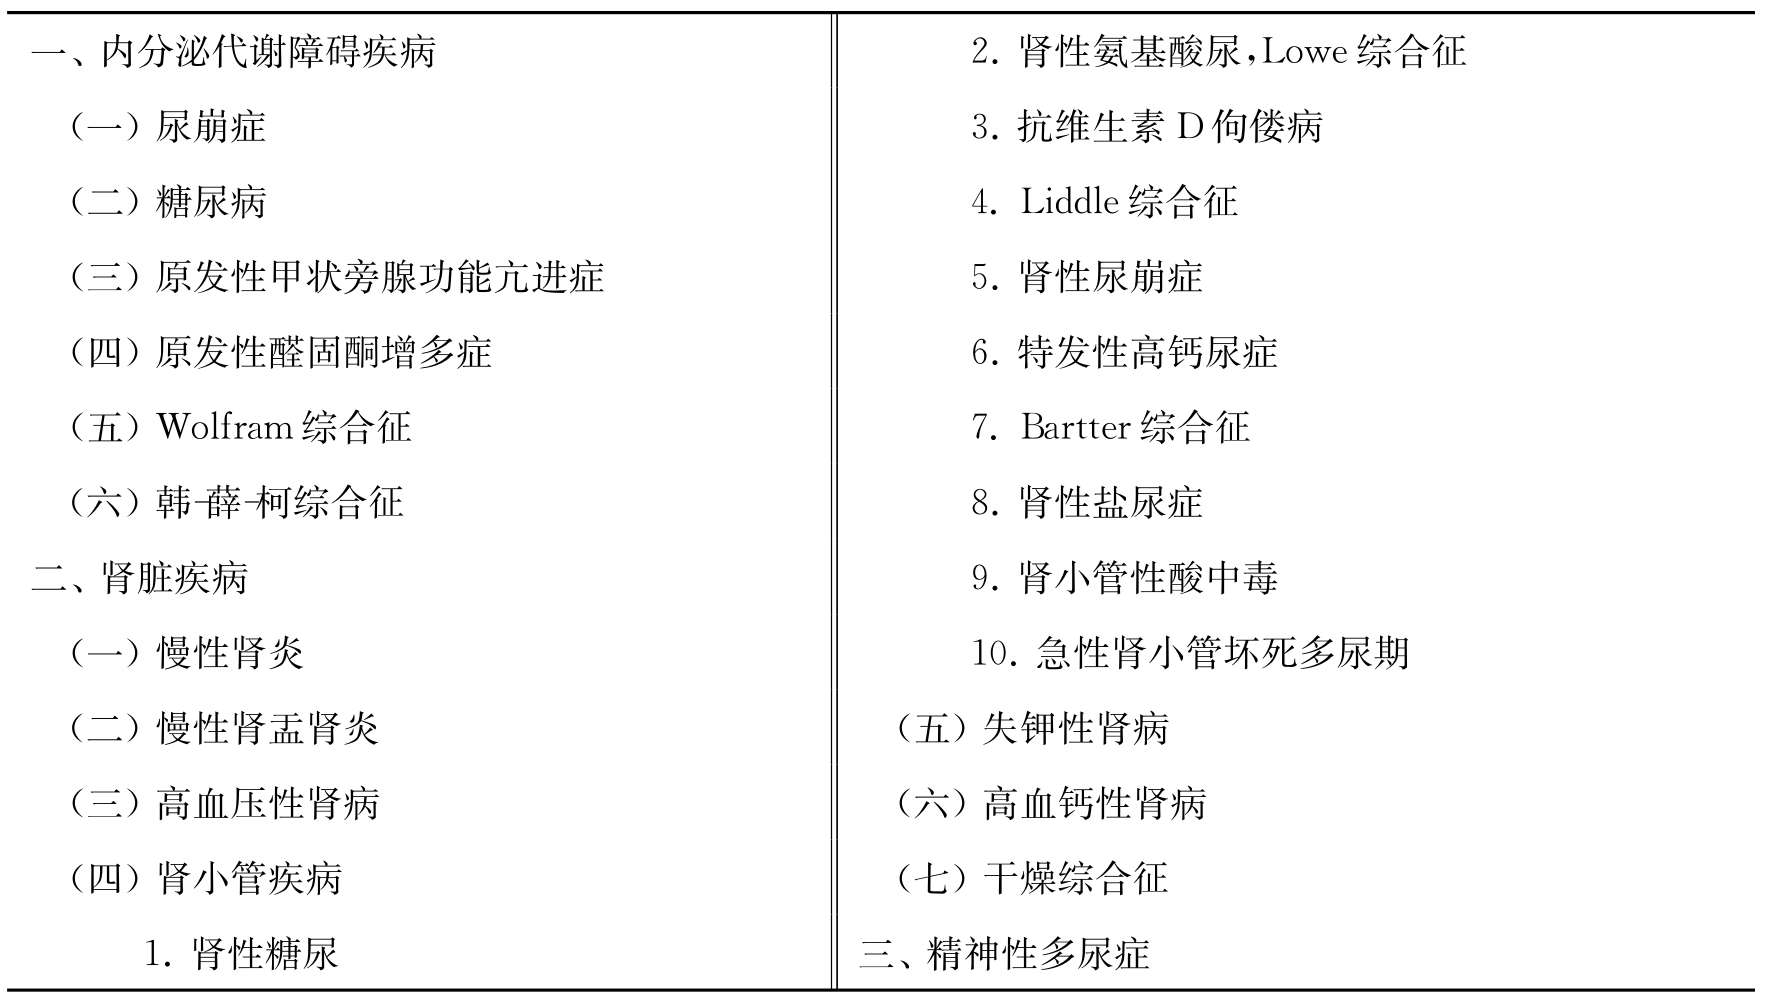
\includegraphics[width=5.88542in,height=3.33333in]{./images/Image00213.jpg}
\end{table}

\subsubsection{(二)肾小管间质功能障碍}

各种原发性或继发性肾小管-间质损害的疾病均可导致多尿。大概与以下因素有关:

1.肾小管对血管升压素反应性降低或无反应,或对某些溶质重吸收的先天或后天性障碍。

2.肾小管、髓袢、肾髓质的高渗功能障碍,以及肾直血管的血循环障碍,影响肾小管浓缩功能。

3.肾小管重吸收碳酸氢盐及(或)酸化尿功能障碍。

\subsubsection{(三)精神、神经性因素}

\subsection{【多尿的诊断与鉴别诊断思路】}

\subsubsection{(一)确定多尿}

准确收集每日总尿量,连续3天,每日总尿量均超过2500ml,可诊断为多尿。但要排除尿频、尿急所致排尿次数增多,其全日总尿量不足2500ml。检查期间要停用利尿剂、输注葡萄糖或其他溶液。

\subsubsection{(二)确定多尿的病因}

一般根据详尽的病史、细致体检及有关的实验室检查,进行综合分析。临床上以多尿为突出症状者,主要是糖尿病、尿崩症、遗传性肾性尿崩症、精神性多饮、多尿症,以及各种原发性或继发性肾小管-间质损害的疾病等。典型的糖尿病症状,尿糖阳性,血糖增高,一般诊断糖尿病不难。精神性多饮、多尿症患者,多为女性,伴有神经症表现,尿量波动大,禁水试验,尿量会逐渐减少,尿比重随即上升(>1.018),渗透压升高,必要时可作高渗盐水试验,若滴注后尿量明显减少,尿比重上升至1.018以上,尿渗透压升高,即可诊断为精神性多饮、多尿症。尿崩症的尿量较多,常达8000~10
000ml以上,饮水量常与尿量相等,尿比重低(1.001~1.005),尿渗透压低(50~200mOsm/L),禁水试验后,尿量不减少,尿比重与渗透压上升不多,一般不会超过1.010,尿渗透压一般不超过血浆渗透压。注射加压素后,则可使尿量明显减少,甚至全部接近正常,尿比重及尿渗透压可进一步升高,但对高渗盐水试验则无反应,或者尿量仅轻度减少(不能减至原来尿量50\%以下)。血浆ADH测定有助于确诊。遗传性肾性尿崩症多尿,患者多从幼年起病,均为男性,临床表现与尿崩症相似,但较轻,多有家族病史,对禁水试验、注射加压素试验和高渗盐水试验均无反应,但血浆ADH明显升高。若为继发于其他各种慢性肾病所致的肾性尿崩症多尿,可根据各种肾病的临床特征,结合注射加压素试验可作出诊断,注射后尿量轻度减少,因继发性者肾小管还可能存在一定的对ADH的反应性。肾小管-间质功能障碍性疾病引起的多尿,有原发性和继发性,除了上述肾性尿崩症外,以多尿为突出症状者有:近端或远端肾小管性酸中毒;约50\%患者有多尿,甚至误认为尿崩症。但本病有高氯性代谢性酸中毒,水、电解质平衡失调,肾结石或肾钙化及(或)肾性骨病等表现,一般诊断不难。肾性糖尿和肾性氨基酸尿虽有多尿表现,但一般不是主要表现。原发性醛固酮增多症患者可有烦渴、多尿,尿量可高达4000ml/d,但患者主要临床表现是高血压、低钾血症、碱血症等,血、尿醛固酮增高,螺内酯试验可使血压下降,血钾恢复正常,B超或CT检查肾上腺可助确诊。甲状旁腺功能亢进引起高血钙性多尿(约1/3病例),不是本病突出症状,主要表现是高血钙、尿路结石、骨质疏松或纤维性骨炎等,仔细检查颈部发现肿大的甲状旁腺可确诊。对于体内有过剩水分须排出的多尿,则有水肿、腹(胸)水等体征或心力衰竭表现,故不难诊断。

本节仅重点讨论某些临床意义较大的疾病。

\paragraph{一、内分泌代谢障碍性疾病}

\subparagraph{(一)尿崩症}

尿崩症是由于下丘脑-神经垂体受损,血管升压素分泌减少或缺乏,以致影响远端肾小管及集合管对水分重吸收而大量排尿所致。病因可分为原发性与继发性两类。原发性病因未明者,其中部分患者证明与遗传有关,可为常染色体显性或伴性遗传。继发性即病因已查出者。在继发性尿崩症中,肿瘤占最多数(52\%),其次为炎症(20\%),如脑炎、脑膜炎、结核、梅毒等,此外为颅外伤(脑震荡、颅底骨折)、脑血管病变、肉芽肿(如嗜酸性肉芽肿、黄脂瘤病、结节病等)、颅内或垂体手术伤及视上-垂体束等。在脑肿瘤中,颅咽管瘤最常见,约有20\%~30\%病例有尿崩症。视交叉部异位松果体瘤则以尿崩症、视力障碍、垂体功能减退及颅内压增高为主要临床特征;发病多在10~20岁,幼年期发病常有性早熟现象,此为早期提示本病的重要线索。黄脂瘤病(韩-薛-柯综合征)国内报告43例中,引起尿崩症者占32.5\%,此外尚有眼球突出、颅骨缺损及肝、脾大等。

一般认为下丘脑损害所致尿崩症较神经垂体受损所引起的严重,因后者需要90\%以上的组织被破坏才会患病,而且还必须在腺垂体、肾上腺皮质和甲状腺功能完整的情况下始能产生尿崩症。当病变进一步侵犯腺垂体而出现腺垂体功能减退时,则尿崩症症状明显减轻或消失。

尿崩症的主要临床特征为多尿,相继引起多饮和烦渴。每日尿量及饮水量多在5升以上,甚至可高达10余升。尿比重低,多为1.000~1.004(如水分补充不足时,尿比重也可达1.010),尿中无其他病理成分。此外,患者常有食欲不振、疲倦乏力、皮肤干燥、口干、便秘、头痛、失眠、精神焦虑、体重减轻以及血钠升高等现象。

根据上述典型表现,一般诊断不难。其特点为:①尿量多,一般4~10L/d。②低比重尿,低渗尿,尿渗透压<血浆渗透压,一般低于200mOsm/L,尿比重多在1.001~1.006,部分性尿崩症患者尿比重可大于1.010,尿渗透压可高于290mOsm/L。③禁水试验不能使尿渗透压和尿比重增加。④ADH或去氨加压素(DDAVP)治疗有明显效果。

尿崩症需与精神性多尿症、遗传性肾性尿崩症相区别。一般根据病史、临床表现即可鉴别(表\ref{tab35-4})。

\begin{table}[htbp]
\centering
\caption{尿崩症与精神性多尿症、遗传性肾性尿崩症的鉴别}
\label{tab35-4}
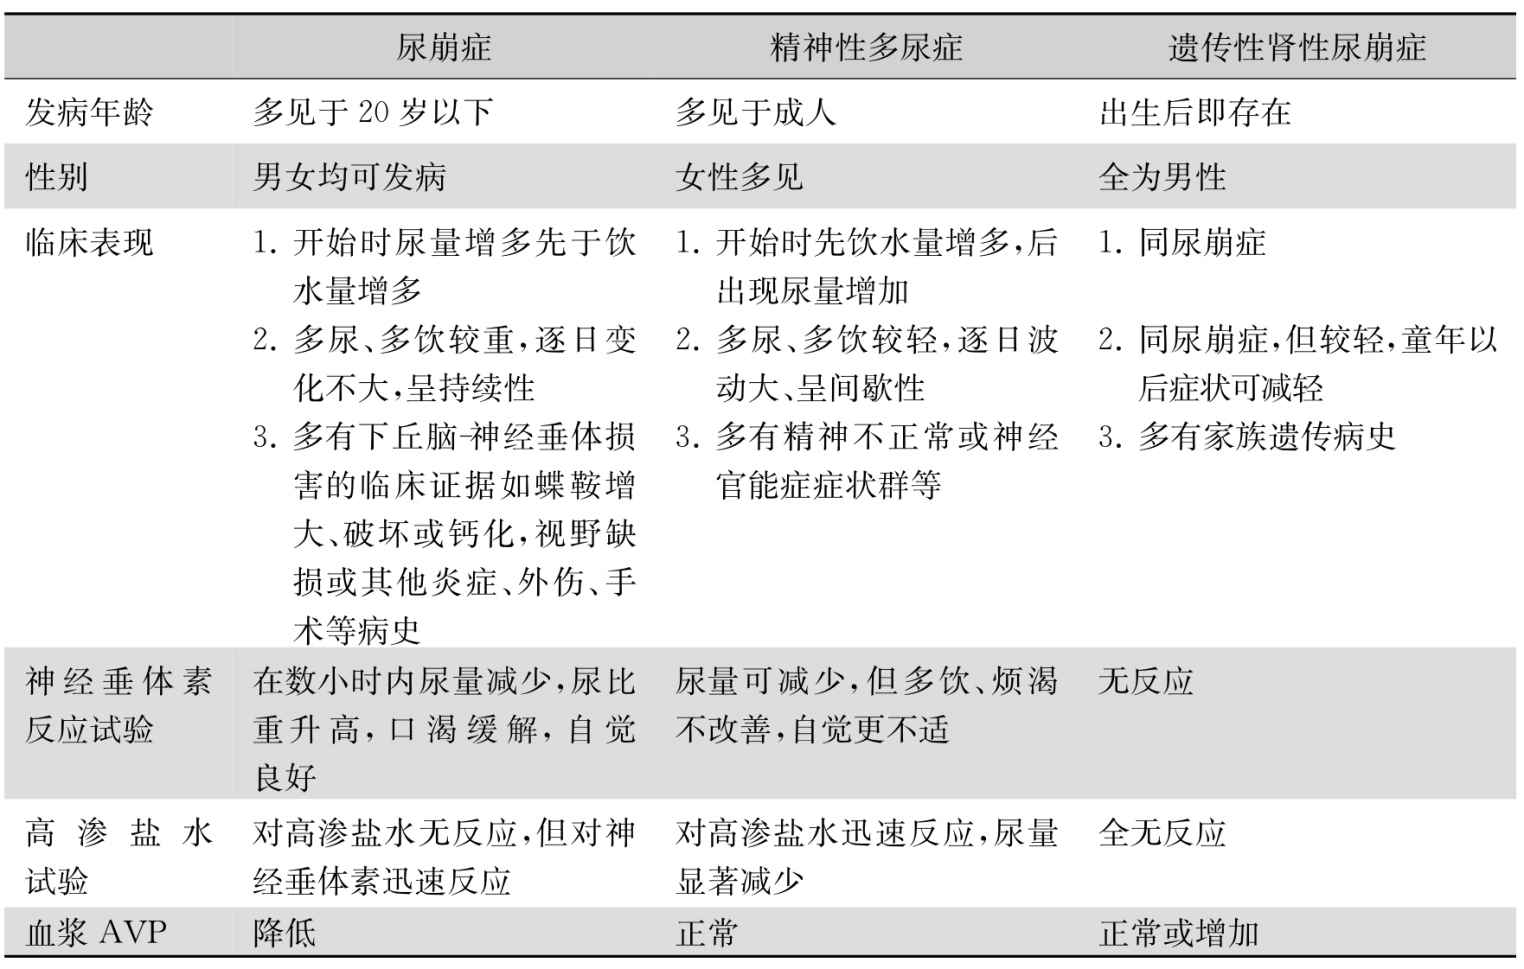
\includegraphics[width=5.86458in,height=3.72917in]{./images/Image00214.jpg}
\end{table}

有时还需进行以下特殊检查以助诊断。

\hypertarget{text00273.htmlux5cux23CHP35-2-2-2-1-1-1}{}
1.血浆精氨酸加压素(AVP)测定

正常人血浆AVP为2.3~7.4pmol/L,禁水后可明显升高。本病患者血AVP减少,禁水后也不增加或增加不明显。

\hypertarget{text00273.htmlux5cux23CHP35-2-2-2-1-1-2}{}
2.血管升压素反应试验

这对尿崩症、精神性多尿症及遗传性肾原性尿崩症三者有鉴别诊断价值。方法:试验前排空膀胱,测定尿量及尿比重,然后肌注长效血管升压素5单位,随之收集数小时尿,并测定尿量及比重。如为尿崩症则尿量迅速显著减少,尿比重增高达1.015以上,烦渴缓解,自觉舒适,但也有少数尿崩症对之无反应;精神性多尿症,尿量也可减少,但烦渴、多饮依旧,自觉更不适;遗传性肾性尿崩症则无反应或反应极微。

\hypertarget{text00273.htmlux5cux23CHP35-2-2-2-1-1-3}{}
3.高渗盐水试验

本试验的目的是提高血浆渗透压,间接测定下丘脑-神经垂体系统分泌血管升压素的能力。这对尿崩症、精神性多尿症及遗传性肾性尿崩症的鉴别诊断有帮助。如为尿崩症,静脉滴注高渗氯化钠溶液后不但尿量不减少,反而增加,只在注射血管升压素后方见减少;在精神性多尿症时,滴注高渗氯化钠溶液后,刺激垂体神经释出血管升压素,而使尿量显著减少;遗传性肾性尿崩症对高渗氯化钠溶液及血管升压素全无反应。

少数精神性多尿症患者,因长期抑制血管升压素的分泌,滴注高渗氯化钠溶液后也不会引起抗利尿反应而呈类似尿崩症的试验结果。此外,严重肾脏病患者对此试验也无明显反应,而类似遗传性肾性尿崩症,有时由于盐渗透性利尿作用,使尿量改变不大或无改变。故在试验时,应辨识此等情况,参考其他材料以进行诊断。

尿崩症有时还须与糖尿病及各种肾脏疾病所致的多尿相鉴别。

尿崩症的诊断确定后,需更进一步找寻病因,如症状出现于脑膜炎、脑炎或颅部外伤之后,则病因大致易于确定。患者有播散性结核病时,提示病因可能为结核性。梅毒病史、血清华氏反应阳性及其他脏器的梅毒性病变,支持病因为梅毒。X线颅骨摄片上有蝶鞍增大、骨质破坏、蝶鞍钙化等征象时,提示尿崩症大约由于蝶鞍部位的肿瘤所致。头颅CT、MRI检查可发现垂体或下丘脑肿瘤。

\subparagraph{(二)糖尿病}

糖尿病患者有尿多和烦渴、多饮的症状,其尿量一般不超过5L/d,并以尿比重高及尿中含糖为特征。国内病例约半数以上有多尿与多饮现象。尿量增加乃是尿中含有糖分以致渗透性利尿的结果,其与糖尿病的严重程度成正比。诊断糖尿病,主要根据其典型症状:即三多(多饮、多尿、多食)、一少(体重减少),以及尿糖阳性、血糖增高等。

部分症状不明显的糖尿病患者,长期未知已罹患本病,致发现此病时往往已有并发症,且常因并发症而进一步检查才发现糖尿病。例如:以白内障、视力减退而就诊于眼科;以反复发作的疖疮或痈而就诊于外科;女性患者则以外阴瘙痒而就诊于妇科;或以四肢麻木、周围神经炎而就诊于神经科。对年龄较轻的冠状动脉硬化性心脏病、抗结核治疗疗效不显著的肺下野或空洞型肺结核、顽固性泌尿道感染、未明原因的肥胖或消瘦等情况,要注意患有糖尿病的可能。

如患者经尿检查发现有葡萄糖尿之后,需测定血糖浓度以证实糖尿病的诊断。正常人空腹血糖值为80~120mg/dl,如有糖尿病症状加上任意时间血浆葡萄糖≥11.1mmol/L
(200mg/dl)或空腹血糖≥7.0mmol/L(126mg/dl)或葡萄糖耐量试验2小时≥11.1mmol/L
(200mg/dl),则糖尿病的诊断可以成立。

\subparagraph{(三)原发性甲状旁腺功能亢进症}

原发性甲状旁腺功能亢进症通常是由于甲状旁腺腺瘤所致,部分也可由于腺体增生或腺癌所致。由于甲状旁腺激素分泌增多,抑制近曲小管重吸收磷酸根,以致磷酸根从尿中排出增多而引起多尿。继之出现口渴、多饮、尿比重偏低。有时被误诊为尿崩症,而不同者乃患者常有骨质疏松、泌尿系结石或顽固性溃疡病等。血钙高、血磷低、血碱性磷酸酶增高、尿磷和尿钙增高也是其特征(参见第131节)。

\subparagraph{(四)原发性醛固酮增多症}

多尿、夜尿和烦渴是原发性醛固酮增多症常见症状,其中以夜尿增多更为突出。多尿的原因主要是由于肾上腺皮质分泌醛固酮增多,作用于远曲小管,而有明显的潴钠排钾作用,血钠增高刺激下视丘烦渴中枢而致烦渴,多饮引起多尿;另一方面也可能由于尿大量排钾,引起失钾性肾病而致多尿。夜尿增多可能与体位有关,因平卧时血管容量扩张,水及盐类排泄增多所致。患者的尿比重较低,一般不超过1.014。本病的诊断根据主要为高血压、低钾血症、肌无力或麻痹、碱血症及血浆容量增多等(参见第40.2节)。

\subparagraph{(五)Wolfram综合征}

本综合征为常染色体隐性遗传病,主要病征为:①糖尿病;②视神经萎缩;③尿崩症;④神经性耳聋。尿崩症为中枢神经性。尿崩症发生率为32\%。

\subparagraph{(六)韩-薛-柯综合征}

本综合征以颅骨破坏、尿崩症和眼球突出为其三大临床特征。报道一组4例中,2例有尿崩症。尿崩症的发病与脑垂体柄或下丘脑受累有关。

\paragraph{二、肾脏疾病}

\subparagraph{(一)慢性肾炎}

慢性肾炎后期由于肾小管浓缩功能减退,故有多尿、夜尿增多、尿比重低(固定于1.010)等表现。

\subparagraph{(二)慢性肾盂肾炎}

慢性肾盂肾炎主要侵犯肾间质,影响肾小管重吸收功能,故可引起多尿与尿比重低,也可引起肾小管性酸中毒、低钾血症等。本病诊断参见第121.1.1节。

\subparagraph{(三)慢性间质性肾炎(CIN)}

病因可多种多样,除全身疾病(如干燥综合征、高尿酸血症等)可继发CIN外,长期接触肾毒性药物、重金属或放射线也可引起慢性间质肾炎。

CIN起病较隐匿,早期有夜尿多尿、肌无力、抽搐、低渗透压尿及低比重尿等肾小管浓缩功能和酸化功能障碍的表现。晚期,肾小球功能受损可出现夜尿、少尿、血肌酐逐渐升高。患者尿常规改变轻微,仅有轻度蛋白尿,少量红、白细胞及管型。对本病的诊断,据临床表现可高度疑诊,但确诊仍常需肾活检病理检查。肾活检主要表现为肾小管萎缩、间质纤维化。

\subparagraph{(四)高血压性肾病}

本病的后期,由于肾浓缩功能减退,可引起多尿、夜尿、低张尿或等张尿等。患者都有长期高血压的病史。

\subparagraph{(五)肾小管疾病}

肾小管疾病是一组以肾小管转运功能缺陷为主要表现的疾病,有的与遗传有关,有的在后天受毒物或炎症损害或免疫反应损伤所引起。临床上常以水、电解质平衡失调、代谢性酸中毒及易发生尿路结石为主要表现;晚期如累及肾小球,则可出现氮质血症等慢性肾衰竭症状。

\hypertarget{text00273.htmlux5cux23CHP35-2-2-2-2-5-1}{}
1.肾性糖尿

肾性糖尿的病因多为原发性,为常染色体隐性遗传病,也可为显性遗传,多有家族史,又称家族性肾性糖尿。偶尔亦可继发于慢性间质性肾炎、肾病综合征、多发性骨髓瘤肾损害等,此时,肾性糖尿多伴有肾小管其他多项转运缺陷。由于近端小管不能将正常滤过的葡萄糖重吸收,于是尿中出现葡萄糖。

绝大多数患者无任何症状,少数可有轻度多饮、多食、多尿、体重减轻。

肾性糖尿的诊断依据:①尿中经常出现尿糖,而血糖正常或偏低,口服糖耐量试验正常,糖贮存及利用正常;②葡萄糖氧化酶试验阳性,显示尿糖为葡萄糖;③无糖尿病和肾脏病证据,肾功能正常;④可有阳性家族史。继发性肾性糖尿除上述特征外,还有原发性肾脏病的特征。遗传性肾性糖尿需与糖尿病鉴别,后者血糖升高,葡萄糖耐量试验异常。

\hypertarget{text00273.htmlux5cux23CHP35-2-2-2-2-5-2}{}
2.肾性氨基酸尿

肾性氨基酸尿是指近端肾小管重吸收氨基酸障碍以致尿中排出大量氨基酸。此类疾病很多,由于氨基酸大量从尿中丢失而引起多尿,但非主要症状。其中主要的疾病有De
Toni-Debré-Fanconi综合征(肾性葡萄糖氨基酸磷酸盐尿)、儿童期发病的Lignac-Fanconi综合征等,是近曲小管对氨基酸、葡萄糖、磷酸盐的重吸收障碍所致。疾病的早期由于上述物质大量从尿中排出而致多尿、等渗尿。此外,患者常有糖尿、代谢性酸中毒、佝偻病(儿童)或软骨病、严重贫血及其他畸形等。

Lowe综合征也是近曲小管对氨基酸、磷酸盐、碳酸氢盐、葡萄糖等重吸收功能障碍所致;除了上述症状外,本病还有眼症状(白内障、青光眼、眼球震颤等)及脑症状(如严重智力发育迟缓、腱反射减弱或消失),故又称为“脑-眼-肾综合征”。

\hypertarget{text00273.htmlux5cux23CHP35-2-2-2-2-5-3}{}
3.抗维生素D佝偻病

此病多为家族性遗传病,由于肾近曲小管对磷酸盐重吸收障碍,而引起多尿,但非主要特征。尿磷增多而血磷降低,以致产生佝偻病,应用一般剂量维生素D治疗无效。本病须与De
Toni-Debré-Fanconi综合征区别,后者尿中有葡萄糖、氨基酸等可作鉴别。

\hypertarget{text00273.htmlux5cux23CHP35-2-2-2-2-5-4}{}
4.Liddle综合征

Liddle综合征(假性醛固酮增多症)为常染色体显性遗传病,甚为罕见。由于远曲小管或集合管不依赖醛固酮的对钠重吸收增加,排钾及H\textsuperscript{+}
增多所致。其特征为高血压、低血钾和碱中毒,多尿、烦渴、肌无力及软瘫,与原发性醛固酮增多症相似,但血及尿中醛固酮水平不高,对醛固酮合成抑制剂或拮抗剂不起反应。给予氨苯蝶啶及补钾盐可改善症状。

在作出诊断之前需排除下述疾病:①原发性醛固酮增多症:其血和尿中醛固酮含量均增高,螺内酯试验阳性。②Bartter综合征:虽有低血钾和碱中毒,但其血压正常,血和尿中醛固酮含量均增加,血浆肾素活性增加,螺内酯试验阳性,肾活检可见肾小球旁器细胞增生。③11-β-羟类固醇脱氢酶缺乏症:其高血压、低血钾性碱中毒与Liddle综合征相似,但尿4-羟皮质醇增多,对螺内酯有反应。

\hypertarget{text00273.htmlux5cux23CHP35-2-2-2-2-5-5}{}
5.肾性尿崩症

肾性尿崩症在临床上罕见,属伴性隐性遗传疾病,亦可继发于某些肾脏病。遗传性的患者均为男性,女性仅能传递此病,是由于远曲小管的先天性缺陷,对血管升压素无应激性能所致。临床症状与垂体性尿崩症完全相同,但血中血管升压素含量正常,对血管升压素无效应。其与尿崩症及精神性多尿症的鉴别诊断,参考表\ref{tab35-4}。

\hypertarget{text00273.htmlux5cux23CHP35-2-2-2-2-5-6}{}
6.特发性高钙尿症

本病尿钙增多,血钙正常,而原因未明,可能与肾曲小管重吸收钙功能障碍及(或)肠道吸收钙亢进以致尿钙增多。典型临床表现:由于尿钙增多,大多数患者有多尿、烦渴、多饮,尿路结石、肾绞痛、血尿等;体内钙呈负平衡,严重者可有骨质疏松,甚至骨软化。诊断主要根据临床表现及尿钙增多(男性>300mg/24小时尿,女性>250mg/24小时尿)。低钙饮食试验(每日摄入钙<300mg,共3日,第4日测24小时尿钙):尿钙排量高于正常。钙耐量试验(低钙低磷饮食3日后,第4日给钙15mg/kg,静脉滴入,于5小时内滴完后第3小时测血钙,并留24小时尿测尿钙):尿钙排量除减去每日基础尿钙排量外,超过滴入钙量的50\%;尿磷排量在滴钙后的第4~12小时较0~4小时降低20\%,表示试验阳性。对诊断有帮助。但必须排除其他引起尿钙增多的疾病如原发性甲状旁腺功能亢进症、肾小管性酸中毒、结节病等。

\hypertarget{text00273.htmlux5cux23CHP35-2-2-2-2-5-7}{}
7.巴特(Bartter)综合征

本病是常染色体隐性遗传病,临床罕见。其发病机制可能是由于肾小管髓袢升支粗段功能障碍,对氯化钠重吸收减少,导致细胞外液量减少,继发高肾素、高醛固酮血症和肾小球旁器增生或肥大。大多数患者表现为多尿、烦渴、夜尿、遗尿及失水。低血钾表现为全身肌无力,但软瘫少见。儿童患者可有特殊容貌如身材矮小、大头、突耳及嘴下翻等,及其他如厌食、嗜盐食、便秘等症状。患者虽有高肾素、高醛固酮血症,但血压正常,无水肿为本病重要特征。

根据低血钾、低血氯、代谢性碱中毒,伴有高肾素、高醛固酮血症,但无高血压及水肿的临床特征,可作初步诊断。肾活检显示肾小球旁器细胞增生和肥大,有助确诊。需与肾小管性酸中毒、原发性醛固酮增多症、Liddle综合征等引起的低钾血症及其他原因引起的低钾血症鉴别,如镁缺乏、使用利尿剂、严重呕吐和腹泻引起的低钾血症和高肾素、高醛固酮血症等(详见有关章节)。

\hypertarget{text00273.htmlux5cux23CHP35-2-2-2-2-5-8}{}
8.失盐性肾炎

失盐性肾炎常继发于慢性肾盂肾炎、肾髓质囊性病、多囊肾、梗阻性肾病等。由于肾小管丧失重吸收钠盐的能力,因而出现多尿。患者突出表现为低钠血症,临床上有乏力、衰弱、低血压、食欲不振、贫血、肌肉抽搐等表现,与慢性肾上腺皮质功能减退症相似,必须注意区别。失盐性肾炎皮肤色素沉着较深,均匀分布,黏膜色素沉着少见,而慢性肾上腺皮质功能减退症色素沉着多见于口腔黏膜及皮肤受压或皱褶处;失盐性肾炎无碳水化合物代谢障碍或低血糖等表现,肾上腺皮质功能正常,尿中17-酮类固醇排量不减少,用去氧皮质酮治疗无效,有助于两者的鉴别。

\hypertarget{text00273.htmlux5cux23CHP35-2-2-2-2-5-9}{}
9.肾小管性酸中毒

肾小管性酸中毒(RTA)是由于肾小管功能不全引起的机体代谢性酸中毒的一种临床综合征。较多见,多数为常染色体显性遗传,也可继发于各种原因的肾小管损害。其临床特征为:高氯性酸中毒,水、电解质紊乱,可有低血钾或高钾血症、低钠血症、低钙血症及多尿、多饮、肾性佝偻病或骨软化症、肾结石等。

临床上可将肾小管酸中毒区分为下列四型:

(1)Ⅰ型肾小管性酸中毒(RTAⅠ):原发性与遗传有关,为常染色体显性遗传,自幼发病。继发性者,最常见于慢性肾小管-间质肾炎,其他先天性遗传性肾脏病如海绵肾、Fabry病、特发性高钙尿症等均可引起。由于远端肾单位功能障碍,排泌H\textsuperscript{+}
和生成氨减少,H\textsuperscript{+}
离子滞留体内,引起酸中毒。加以Cl\textsuperscript{-}
排泄减少,肾小管重吸收NaCl增多,Na\textsuperscript{+}
-K\textsuperscript{+} 离子交换增多,致K\textsuperscript{+}
大量丧失,引起低钾血症与高氯血症性酸中毒。此型临床上最多见,可发生于任何年龄,但以20~40岁之间出现症状者较多。临床表现有疲乏,烦渴、多尿、全身骨痛以及肌肉乏力、软瘫、骨质疏松、病理性骨折和尿钙增多所致尿路结石形成等。由于临床表现往往与尿崩症、类风湿关节炎、神经肌肉疾病、周期性瘫痪等相似,易致误诊与漏诊。根据上述临床表现及高氯低钾血症性代谢性酸中毒,而尿pH不能降至6.0以下,则可确诊。轻型者可作氯化铵负荷试验[停用碱性药物2~3天,口服氯化铵0.1g/(kg·d),分3~4次服,连服3天],试验后血pH
或CO2CP降低(pH<7.34,或CO\textsubscript{2}
CP≤20mmol/L,而尿pH不能降至5.5以下,有助确诊。

(2)Ⅱ型肾小管性酸中毒(RTAⅡ):本型系由于近端肾小管对\ce{HCO3-}
的重吸收缺陷引起;大量\ce{HCO3-}
的丢失引起高氯血症性酸中毒。原发性者大多数为男性儿童,多伴有其他肾小管缺陷。主要表现为生长发育障碍(由于酸中毒),可有低血钾症状(肌无力、多尿、烦渴、多饮)。或有继发性醛固酮增多、骨质疏松、骨软化等,通常只有轻度高钙尿症,罕有结石形成。继发性者常有其他肾小管缺陷,形成范可尼综合征。重症者可表现为高血氯性酸中毒。因远端肾小管酸化功能正常,氯化铵负荷试验时尿pH可<5.5。根据患者的临床表现和实验室检查,一般诊断不难。确诊可作碳酸氢盐重吸收试验。给患者口服或静脉滴注碳酸氢钠,纠正血浆\ce{HCO3-}
浓度至正常,测定尿\ce{HCO3-}
排量,及计算滤过的\ce{HCO3-}
排泄率,如尿\ce{HCO3-}
排泄率大于滤过量的15\%,则可确诊。

(3)Ⅲ型肾小管性酸中毒(RTAⅢ):本型兼有近端和远端肾小管功能障碍,故兼有Ⅰ型和Ⅱ型的表现,症状较严重,高血氯性酸中毒明显,尿中大量\ce{HCO3-}
丢失,尿可滴定酸和铵排出减少。从尿中丢失的\ce{HCO3-}
约占肾小球滤出量的5\%~10\%左右。

(4)Ⅳ型肾小管性酸中毒(RTAⅣ):本型RTA又称高血钾型远端肾小管性酸中毒,由于醛固酮不足或对醛固酮拮抗,远端肾小管排泌H\textsuperscript{+}
、K\textsuperscript{+}
减少,故发生酸中毒和高钾血症。多伴有低肾素、低醛固酮血症。因常有轻、中度氮质血症,需与肾小球功能不全所致的酸中毒鉴别,本病的酸中毒和高钾血症较重,与GFR降低程度不平行,可作鉴别。

\hypertarget{text00273.htmlux5cux23CHP35-2-2-2-2-5-10}{}
10.急性肾小管坏死多尿期

急性肾小管坏死经过10~14天的少尿期后,每天尿量可达数升(参见本章上文)。

\subparagraph{(六)失钾性肾病}

本病主要是由于长期而严重的失钾(如胃肠道失钾、肾性失钾等)所致,严重的低钾可使肾小管上皮细胞空泡变性,肾浓缩功能降低,出现明显的夜尿、多尿及烦渴,严重者可出现肾性尿崩症,对血管升压素反应不佳。部分患者由于肾间质损害还可引起肾小管性酸中毒,此外,患者常有低钾血症的一系列临床表现。

根据上述症状,结合原发病史,一般即可成立诊断。此病常需与原发性醛固酮增多症鉴别,因两者均可出现多尿、多饮、低钾血症等,但后者有高血压、碱血症、血容量增高等以助鉴别。

\subparagraph{(七)高血钙性肾病}

此病是由于长期血钙增高所致的肾损害及肾功能障碍。主要的病理改变是远曲管及集合管细胞变性、坏死和钙化,严重者肾间质、肾小球或血管钙化导致瘢痕形成及肾硬化。引起高血钙的病因主要有:甲状旁腺功能亢进症、结节病、维生素D中毒症、多发性骨髓瘤、转移性恶性骨瘤等。

早期主要表现为肾脏浓缩功能减退,患者出现多尿、夜尿、烦渴、尿比重和尿渗透压降低,甚至可发生肾性尿崩症,此外,患者有血钙增高(>2.75mmol/L)和尿钙增多,常有肾钙化或肾结石,容易发生尿路感染。晚期病变累及肾小球,可出现进行性肾功能不全。

根据上述临床表现,结合原发病特征,一般即可确立诊断。

\paragraph{三、精神性多尿症}

本症的烦渴、多饮、多尿为暂时性,多尿是由于狂饮所致,尿量每日2~5L不等。临床上尚可发现其他神经症症状。患者较能耐受口渴,此时排尿量可相对减少,而尿比重可升高至1.015以上。尿崩症患者停止饮水时,出现极度烦渴、神经过敏、虚弱与体温过低,而仍继续排出大量低比重尿。高渗盐水试验对两者鉴别帮助较大。此外,尚需与遗传性肾性尿崩症鉴别。

\protect\hypertarget{text00274.html}{}{}

\section{参考文献}

少尿或无尿

1.黄兴,等.成人原发性肾小球疾病205例的临床与病理.中华肾脏病杂志,1995,11(5):297

2.章友康,谌贻璞.肾脏病学1997年进展.中华医学杂志,1997,77(12):887

3.郑法雷.药物性肾损害.中华内科杂志,1996,35(9):642

4.余英豪,等.肾小管间质疾病新分类法.中华肾脏病杂志,1994,10(1):55

5.陈惠萍,等.急性间质性肾炎的临床与病理研究.中华肾脏病杂志,1994,10(5):284

6.章友康,赵明辉.原发性小血管炎及其肾损伤的治疗.中华肾脏病杂志,1998,14(1):58

7.魏林,等.原发性小血管炎肾损害(综述).中华肾脏病杂志,1996,12(1):56

8.孙志熙,等.肾后性肾功能衰竭的诊断和治疗.中华外科杂志,1997,35(8):501

9.尹广,黎磊石.药物性间质性肾炎的临床及病理研究.中华肾脏病杂志,1997,13(2):833

10.史继学.静脉滴注20\%甘露醇诱发急性肾损害12例.中华内科杂志,1996,35(6):381

11.周福德,等.中草药引起的肾损害.中华肾脏病杂志,1996,12(1):54

12.许国章.药物引起免疫性肾小管间质性肾炎.中华内科杂志,1996,335(6):422

13.卢延,等.磁共振泌尿道造影对泌尿道扩张及梗阻的诊断价值.中华医学杂志,1998,78(9):670

14.李寒,等.急性肾功能衰竭为首发表现的多发性骨髓瘤.中华老年多器官疾病杂志,2003,2(2):143

15.杨焕荣,等.新型隐球菌致急性间质性肾炎一例.中华肾脏病杂志,2002,18(2):126

多 尿

1.胡曼东.21例干燥综合征的肾损害分析.中华肾脏病杂志,1998,14(2):130

2.石长虹,等.母女同患Wolfram综合征二例.中华内分泌代谢杂志,1998,14(2):92

3.江水娣,等.Bartter综合征的诊断和治疗(附4例报告).中华内分泌代谢杂志,1995,11(1):57

4.陈有才,等.遗传性垂体性尿崩症一个家系分析.中华内分泌代谢杂志,1997,13(4):253

5.周浩,等.抗结核药引起多尿一例.中华内科杂志,2001,40(7):441

6.章振林,田慧.骨痛、乏力、多饮、多尿20年.中华内分泌代谢杂志,2000,16(1):58

7.崔义才,董俊玲.躁狂症伴多饮多尿一例.中华精神科杂志,1999,32(2):111

\protect\hypertarget{text00275.html}{}{}

